\documentclass[nooutcomes]{ximera}
\input{../preamble.tex}


\author{Elizabeth Miller, Kenneth Berglund}
%\license{Creative Commons 4.0 International License}



\title{Famous Function Properties}

\begin{document}

\begin{abstract}
\end{abstract}
\maketitle

%\typeout{************************************************}
%\typeout{Famous Functions and Relations}
%\typeout{************************************************}

%\section{Famous Functions and Relations} 
In Section 1-2, you saw a variety of famous functions. Now that we have learned more about properties of functions, we can update our knowledge of those famous functions. We will go through the list of famous functions from before and point out where each function might have properties we've since discussed.

\newpage

%\typeout{************************************************}
%\typeout{Linear Functions}
%\typeout{************************************************}

\section{Linear Functions}
Recall that the graph of a linear function is a line. 

\begin{example}
A prototypical example of a linear function is $$ \mbox{\huge $y=x.$}$$ 

\begin{image}
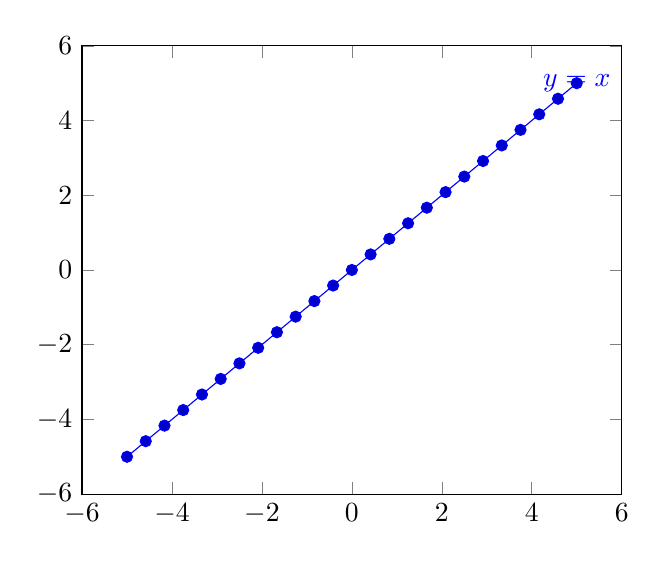
\begin{tikzpicture}
    \begin{axis}
        \addplot{x} node{$y=x$};
    \end{axis}
\end{tikzpicture}
\end{image}

\begin{center}
\(
\begin{array}{ |c || c|  }
 \hline
 \multicolumn{2}{|c|}{\text{\normalfont Important Values of } y=x} \\
\hline
 \hline
 x & y\\
 \hline
 -2&-2\\
 -1&-1\\
 0&0\\
 1&1\\
 2&2\\
 \hline
\end{array}
\)
\end{center}
\end{example}

In general, linear functions can be written as $y=mx+b$ where $m$ and $b$ can be any numbers. We learned that $m$ represents the slope, and $b$ is the $y$-coordinate of the $y$-intercept. You can play with changing the values of $m$ and $b$ on the graph using Desmos and see how that changes the line.  

\begin{center}  
\desmos{japnhapzvn}{800}{600}  
\end{center}

Note that a linear function $f$ defined by $f(x) = mx + b$ with $b = 0$ is odd. If $m = 0$, then $f$ is periodic, since it is constant. Furthermore, constant functions are always even.

Additionally, if $m \ne 0$, then a linear function is one-to-one, and therefore invertible. We summarize this information in the table below.

\begin{center}
$
\begin{array}{|l|l|}
 \hline
 \multicolumn{2}{|c|}{\text{\normalfont Properties of Linear Functions } y=mx + b} \\
\hline
 \hline
\text{Periodic?} & \text{If } m = 0 \\ \hline
\text{Odd?} & \text{If } b = 0 \\ \hline
\text{Even?} & \text{If } m = 0 \\ \hline
\text{One-to-one/invertible?} & \text{Yes}\\ \hline
\end{array}
$
\end{center}

\newpage

%\typeout{************************************************}
%\typeout{Quadratic Functions}
%\typeout{************************************************}

\section{Quadratic Functions}

Recall that the graph of a quadratic function is a parabola.

\begin{example}
A prototypical example of a quadratic function is $$ \mbox{\huge $y=x^2.$}$$

\begin{image}
\begin{tikzpicture}
    \begin{axis}
        \addplot[smooth]{x^2} node{$y=x^2$};
    \end{axis}
\end{tikzpicture}
\end{image}

\begin{center}
\(
\begin{array}{ |c || c|  }
 \hline
 \multicolumn{2}{|c|}{\text{\normalfont Important Values of } y=x^2} \\
\hline
 \hline
 x & y\\
 \hline
 -2&4\\
 -1&1\\
 0&0\\
 1&1\\
 2&4\\
 \hline
\end{array}
\)
\end{center}
\end{example}

In general, quadratic functions can be written as $y=ax^2+bx+c$ where $a$, $b$, and $c$ can be any numbers.  You can play with changing the values of $a$, $b$, and $c$ on the graph using Desmos and see how that changes the parabola.  

\begin{center}  
\desmos{nmlghfrws9}{800}{600}  
\end{center}

Note that for a quadratic function $f$ defined by $f(x) = ax^2 + bx + c$, if $b = 0$, then $f$ is even. In general, quadratic functions are not one-to-one, odd, or periodic, except in cases where $a = 0$, in which we're actually dealing with a linear function. We summarize this information in the table below.

\begin{center}
$
\begin{array}{|l|l|}
 \hline
 \multicolumn{2}{|c|}{\text{\normalfont Properties of Quadratic Functions } y=ax^2 + bx + c, a \ne 0} \\
\hline
 \hline
\text{Periodic?} & \text{No} \\ \hline
\text{Odd?} & \text{No} \\ \hline
\text{Even?} & \text{If } b = 0 \\ \hline
\text{One-to-one/invertible?} & \text{No}\\ \hline
\end{array}
$
\end{center}

\newpage

%\typeout{************************************************}
%\typeout{Absolute Value}
%\typeout{************************************************}

\section{Absolute Value}
Another important type of function is the absolute value function.  This is the function that takes all $y$-values and makes them positive.  The absolute value function is written as 

$$ \mbox{\huge $y=|x|.$}$$ 

\begin{image}
\begin{tikzpicture}
    \begin{axis}
        \addplot[smooth]{abs(x)} node{$y=|x|$};
    \end{axis}
\end{tikzpicture}
\end{image}

\begin{center}
\(
\begin{array}{ |c || c|  }
 \hline
 \multicolumn{2}{|c|}{\text{\normalfont Important Values of } y=|x|} \\
\hline
 \hline
 x & y\\
 \hline
 -2&2\\ 
-1&1\\ 
0&0\\
 1&1\\
 2&2\\
 \hline
\end{array}
\)
\end{center}

Notice that the absolute value function is even. Is it one-to-one? The fact that it's even tells us that it is not, since $|-x| = |x|$ for all $x$. We summarize this information in the table below.

\begin{center}
$
\begin{array}{|l|l|}
 \hline
 \multicolumn{2}{|c|}{\text{\normalfont Properties of the Absolute Value Function } y=|x|} \\
\hline
 \hline
\text{Periodic?} & \text{No} \\ \hline
\text{Odd?} & \text{No} \\ \hline
\text{Even?} & \text{Yes } \\ \hline
\text{One-to-one/invertible?} & \text{No}\\ \hline
\end{array}
$
\end{center}

\newpage

%\typeout{************************************************}
%\typeout{Square Root}
%\typeout{************************************************}

\section{Square Root}
Another famous function is the square root function, $$ \mbox{\huge $y=\sqrt{x}.$}$$ 

\begin{image}
\begin{tikzpicture}
    \begin{axis}
        \addplot[samples=200,domain=0:30]{sqrt(x)};
    \end{axis}
\end{tikzpicture}
\end{image}


\begin{center}
\(
\begin{array}{ |c || c|  }
 \hline
 \multicolumn{2}{|c|}{\text{\normalfont Important Values of } y=\sqrt{x}} \\
\hline
 \hline
 x & y\\
 \hline
 0&0\\
 1&1\\
 4&2\\
 9&3\\
 25&5\\
 \hline
\end{array}
\)
\end{center}

The square root function is one-to-one. Negative inputs are not valid for the square root function, so it is neither even, odd, nor periodic. We summarize this information in the table below.

\begin{center}
$
\begin{array}{|l|l|}
 \hline
 \multicolumn{2}{|c|}{\text{\normalfont Properties of the Square Root Function } y=\sqrt{x}} \\
\hline
 \hline
\text{Periodic?} & \text{No} \\ \hline
\text{Odd?} & \text{No} \\ \hline
\text{Even?} & \text{No} \\ \hline
\text{One-to-one/invertible?} & \text{Yes}\\ \hline
\end{array}
$
\end{center}

\newpage

%\typeout{************************************************}
%\typeout{Exponential}
%\typeout{************************************************}

\section{Exponential}
Another famous function is the exponential growth function, $$ \mbox{\huge $y=e^{x}.$}$$ 

Here $e$ is the mathematical constant known as Euler's number.  $e \approx 2.71828 .$.

\begin{image}
\begin{tikzpicture}
    \begin{axis}
        \addplot[samples=200,domain=-10:4]{e^x};
    \end{axis}
\end{tikzpicture}
\end{image}

\begin{center}
\(
\begin{array}{ |c || c|  }
 \hline
 \multicolumn{2}{|c|}{\text{\normalfont Important Values of } y=e^x} \\
\hline
 \hline
 x & y\\
 \hline
 0&1\\[2ex]
 1&e\\[2ex]
 -1&\frac{1}{e}\\[2ex]
 \hline
\end{array}
\)
\end{center}

In general, we can talk about exponential functions of the form $y=b^{x}$ where $b$ is a positive number not equal to $1$.  You can play with changing the values of $b$ on the graph using Desmos and see how that changes the graph.  Pay particular attention to the difference between $b>1$ and $0<b<1$.

\begin{center}  
%\desmos{dgcwh0chfv}{800}{600}  
\desmos{qsmvb7tiex}{800}{600}
\end{center}

Notice that exponential functions are one-to-one, and therefore invertible. However, they are neither even, odd, nor periodic. We summarize this information in the table below.

\begin{center}
$
\begin{array}{|l|l|}
 \hline
 \multicolumn{2}{|c|}{\text{\normalfont Properties of the Exponential Functions } y=b^x} \\
\hline
 \hline
\text{Periodic?} & \text{No} \\ \hline
\text{Odd?} & \text{No} \\ \hline
\text{Even?} & \text{No} \\ \hline
\text{One-to-one/invertible?} & \text{Yes} \\ \hline
\end{array}
$
\end{center}


\newpage

%\typeout{************************************************}
%\typeout{Logarithms}
%\typeout{************************************************}

\section{Logarithm}
Another group of famous functions are logarithms.

\begin{example}
The most famous logarithm function is
 $$ \mbox{\huge $y=\ln(x)=\log_{e}(x)$.}$$ 
Here $e$ is the mathematical constant known as Euler's number. $e \approx 2.71828$.

\begin{image}
\begin{tikzpicture}
    \begin{axis}
        \addplot[samples=200,domain=0.01:8]{ln(x)};
    \end{axis}
\end{tikzpicture}
\end{image}

\begin{center}
\(
\begin{array}{ |c || c|  }
 \hline
 \multicolumn{2}{|c|}{\text{\normalfont Important Values of } y=ln(x)} \\
\hline
 \hline
 x & y\\
 \hline
0&\text{\normalfont undefined}\\ 
\frac{1}{e}&-1\\ [2ex]
1&0\\[2ex]
 e&1\\[2ex]
 \hline
\end{array}
\)
\end{center}

\end{example}

You may notice that the table of values for $y=\ln(x)$ and $y=e^x$ are similiar.  This is becase these two functions are interconnected.  We will explore this more later in the course.

In general, we can talk about logarithmic functions of the form $y=\log_b(x)$ where $b$ is a positive number not equal to $1$.  You can play with changing the values of $b$ on the graph using Desmos and see how that changes the graph.  Pay particular attention to the difference between $b>1$ and $0<b<1$.

\begin{center}  
\desmos{lxllnpdi6w}{800}{600}  
\end{center}

Notice that logarithms are neither even, odd, nor periodic. However, they are one-to-one, and therefore invertible. It turns out that the inverse of a logarithm is an exponential function, and vice versa! We summarize this information in the table below.

\begin{center}
$
\begin{array}{|l|l|}
 \hline
 \multicolumn{2}{|c|}{\text{\normalfont Properties of the Logarithm Functions } y=\log_b(x)} \\
\hline
 \hline
\text{Periodic?} & \text{No} \\ \hline
\text{Odd?} & \text{No} \\ \hline
\text{Even?} & \text{No} \\ \hline
\text{One-to-one/invertible?} & \text{Yes} \\ \hline
\end{array}
$
\end{center}

\newpage

%\typeout{************************************************}
%\typeout{Sine}
%\typeout{************************************************}

\section{Sine}
Another important function is the sine function, $$ \mbox{\huge $y=\sin(x)$.}$$ 


This function comes from trigonometry. In the table below we will use another mathematical constant, $\pi$ (``pi" pronounced pie). $\pi \approx 3.14159$.

\begin{image}
\begin{tikzpicture}
    \begin{axis}[ymin=-2, ymax=2,
		   %xtick={-6.28318, -4.7123889, -3.14159, -1.5708, 1.5708, 3.14159, 4.7123889, 6.28318},
    xticklabels={
        $-\frac{3\pi}{2}$, $-\pi$, $\frac{\pi}{2}$, $0$,
        $\frac{\pi}{2}$, $\pi$, $\frac{3\pi}{2}$, $2\pi$
    }, ]
        \addplot[samples=200]{sin(pi/4*deg(x))};
    \end{axis}
\end{tikzpicture}
\end{image}

\begin{center}
\(
\begin{array}{ |c || c|  }
 \hline
 \multicolumn{2}{|c|}{\text{\normalfont Important Values of } y=\sin(x)} \\
\hline
 \hline
 x & y\\
 \hline

 -\pi&0\\

 -\frac{\pi}{2}&-1\\[2ex]

 0&0\\

 \frac{\pi}{2}&1\\[2ex]

 \pi&0\\

\frac{3\pi}{2}&-1\\[2ex]

 2 \pi&0\\
\hline
\end{array}
\)
\end{center}

As mentioned earlier, the sine function is odd and periodic with period $2\pi$. Since it is periodic, however, it cannot be one-to-one, since its values repeat. We summarize this information in the table below.

\begin{center}
$
\begin{array}{|l|l|}
 \hline
 \multicolumn{2}{|c|}{\text{\normalfont Properties of the Sine Function } y=\sin(x)} \\
\hline
 \hline
\text{Periodic?} & \text{Yes, with period }2\pi \\ \hline
\text{Odd?} & \text{Yes} \\ \hline
\text{Even?} & \text{No} \\ \hline
\text{One-to-one/invertible?} & \text{No} \\ \hline
\end{array}
$
\end{center}

In general, we can consider $y=a\sin(bx)$.  You can play with changing the values of $a$ and $b$ on the graph using Desmos and see how that changes the graph.  

\begin{center}  
\desmos{vkxzcfv2aq}{800}{600}  
\end{center}



\newpage

%\typeout{************************************************}
%\typeout{Cosine}
%\typeout{************************************************}

\section{Cosine}
A function introduced in Section 3-2 is the cosine function, $$ \mbox{\huge $y=\cos(x)$.}$$ 


As with sine, the cosine function comes from trigonometry. In the table below we will again use $\pi$.

\begin{image}
\begin{tikzpicture}
    \begin{axis}[ymin=-2, ymax=2,
		   %xtick={-6.28318, -4.7123889, -3.14159, -1.5708, 1.5708, 3.14159, 4.7123889, 6.28318},
    xticklabels={
        $-\frac{3\pi}{2}$, $-\pi$, $\frac{\pi}{2}$, $0$,
        $\frac{\pi}{2}$, $\pi$, $\frac{3\pi}{2}$, $2\pi$
    }, ]
        \addplot[samples=200]{cos(pi/4*deg(x))};
    \end{axis}
\end{tikzpicture}
\end{image}

\begin{center}
\(
\begin{array}{ |c || c|  }
 \hline
 \multicolumn{2}{|c|}{\text{\normalfont Important Values of } y=\cos(x)} \\
\hline
 \hline
 x & y\\
 \hline

 -\pi&-1\\

 -\frac{\pi}{2}&0\\[2ex]

 0&1\\

 \frac{\pi}{2}&0\\[2ex]

 \pi&-1\\

\frac{3\pi}{2}&0\\[2ex]

 2 \pi&1\\
\hline
\end{array}
\)
\end{center} 

As mentioned earlier, the cosine function is even and periodic with period $2\pi$. Since it is periodic, however, it cannot be one-to-one, since its values repeat. We summarize some information in the table below.

\begin{center}
$
\begin{array}{|l|l|}
 \hline
 \multicolumn{2}{|c|}{\text{\normalfont Properties of the Cosine Function } y=\cos(x)} \\
\hline
 \hline
\text{Periodic?} & \text{Yes, with period }2\pi \\ \hline
\text{Odd?} & \text{No} \\ \hline
\text{Even?} & \text{Yes} \\ \hline
\text{One-to-one/invertible?} & \text{No} \\ \hline
\end{array}
$
\end{center}

In general, we can consider $y=a\cos(bx)$.  You can play with changing the values of $a$ and $b$ on the graph using Desmos and see how that changes the graph.  

\begin{center}  
\desmos{kvmz1kt19n}{800}{600}  
\end{center}




\end{document}
